\documentclass{article}

% Packages required to support encoding
\usepackage{ucs}
\usepackage[utf8x]{inputenc}
\usepackage{graphicx} 
% Packages required by code

% Packages always used
\usepackage{listings}
\usepackage{hyperref}
\usepackage{xspace}
\usepackage[usenames,dvipsnames]{color}
\hypersetup{colorlinks=true,urlcolor=blue}
\usepackage{multicol}

\usepackage[framed,numbered,autolinebreaks,useliterate] {mcode}


\usepackage{geometry}
\geometry{letterpaper,textwidth=350pt,textheight=680pt,tmargin=60pt,
            left=72pt,footskip=24pt,headsep=18pt,headheight=14pt}
\usepackage{amsmath}
\usepackage{amssymb}
\usepackage{textcase}
\usepackage{soul}

\newcommand{\mat}[1]{\boldsymbol{#1}}\renewcommand{\vec}[1]{\boldsymbol{\mathrm{#1}}}
\newcommand{\vecalt}[1]{\boldsymbol{#1}}

\newcommand{\conj}[1]{\overline{#1}}

\newcommand{\normof}[1]{\|#1\|}
\newcommand{\onormof}[2]{\|#1\|_{#2}}

\newcommand{\itr}[2]{#1^{(#2)}}
\newcommand{\itn}[1]{^{(#1)}}

\newcommand{\eps}{\varepsilon}
\newcommand{\kron}{\otimes}

\DeclareMathOperator{\diag}{diag}
\DeclareMathOperator{\trace}{trace}
\DeclareMathOperator{\tvec}{vec}

\newcommand{\prob}{\mathbb{P}}
\newcommand{\probof}[1]{\prob\left\{ #1 \right\}}

\newcommand{\pmat}[1]{\begin{pmatrix} #1 \end{pmatrix}}
\newcommand{\bmat}[1]{\begin{bmatrix} #1 \end{bmatrix}}
\newcommand{\spmat}[1]{\left(\begin{smallmatrix} #1 \end{smallmatrix}\right)}
\newcommand{\sbmat}[1]{\left[\begin{smallmatrix} #1 \end{smallmatrix}\right]}

\newcommand{\RR}{\mathbb{R}}
\newcommand{\CC}{\mathbb{C}}

\providecommand{\eye}{\mat{I}}
\providecommand{\mA}{\ensuremath{\mat{A}}}
\providecommand{\mB}{\ensuremath{\mat{B}}}
\providecommand{\mC}{\ensuremath{\mat{C}}}
\providecommand{\mD}{\ensuremath{\mat{D}}}
\providecommand{\mE}{\ensuremath{\mat{E}}}
\providecommand{\mF}{\ensuremath{\mat{F}}}
\providecommand{\mG}{\ensuremath{\mat{G}}}
\providecommand{\mH}{\ensuremath{\mat{H}}}
\providecommand{\mI}{\ensuremath{\mat{I}}}
\providecommand{\mJ}{\ensuremath{\mat{J}}}
\providecommand{\mK}{\ensuremath{\mat{K}}}
\providecommand{\mL}{\ensuremath{\mat{L}}}
\providecommand{\mM}{\ensuremath{\mat{M}}}
\providecommand{\mN}{\ensuremath{\mat{N}}}
\providecommand{\mO}{\ensuremath{\mat{O}}}
\providecommand{\mP}{\ensuremath{\mat{P}}}
\providecommand{\mQ}{\ensuremath{\mat{Q}}}
\providecommand{\mR}{\ensuremath{\mat{R}}}
\providecommand{\mS}{\ensuremath{\mat{S}}}
\providecommand{\mT}{\ensuremath{\mat{T}}}
\providecommand{\mU}{\ensuremath{\mat{U}}}
\providecommand{\mV}{\ensuremath{\mat{V}}}
\providecommand{\mW}{\ensuremath{\mat{W}}}
\providecommand{\mX}{\ensuremath{\mat{X}}}
\providecommand{\mY}{\ensuremath{\mat{Y}}}
\providecommand{\mZ}{\ensuremath{\mat{Z}}}
\providecommand{\mLambda}{\ensuremath{\mat{\Lambda}}}
\providecommand{\mPbar}{\bar{\mP}}

\providecommand{\ones}{\vec{e}}
\providecommand{\va}{\ensuremath{\vec{a}}}
\providecommand{\vb}{\ensuremath{\vec{b}}}
\providecommand{\vc}{\ensuremath{\vec{c}}}
\providecommand{\vd}{\ensuremath{\vec{d}}}
\providecommand{\ve}{\ensuremath{\vec{e}}}
\providecommand{\vf}{\ensuremath{\vec{f}}}
\providecommand{\vg}{\ensuremath{\vec{g}}}
\providecommand{\vh}{\ensuremath{\vec{h}}}
\providecommand{\vi}{\ensuremath{\vec{i}}}
\providecommand{\vj}{\ensuremath{\vec{j}}}
\providecommand{\vk}{\ensuremath{\vec{k}}}
\providecommand{\vl}{\ensuremath{\vec{l}}}
\providecommand{\vm}{\ensuremath{\vec{l}}}
\providecommand{\vn}{\ensuremath{\vec{n}}}
\providecommand{\vo}{\ensuremath{\vec{o}}}
\providecommand{\vp}{\ensuremath{\vec{p}}}
\providecommand{\vq}{\ensuremath{\vec{q}}}
\providecommand{\vr}{\ensuremath{\vec{r}}}
\providecommand{\vs}{\ensuremath{\vec{s}}}
\providecommand{\vt}{\ensuremath{\vec{t}}}
\providecommand{\vu}{\ensuremath{\vec{u}}}
\providecommand{\vv}{\ensuremath{\vec{v}}}
\providecommand{\vw}{\ensuremath{\vec{w}}}
\providecommand{\vx}{\ensuremath{\vec{x}}}
\providecommand{\vy}{\ensuremath{\vec{y}}}
\providecommand{\vz}{\ensuremath{\vec{z}}}
\providecommand{\vpi}{\ensuremath{\vecalt{\pi}}}

\sodef\allcapsspacing{\upshape}{0.15em}{0.65em}{0.6em}%

\makeatletter
\def\maketitle{%
\par
\hrule height 0.75pt\vspace{1ex}
\par\noindent
\begin{minipage}{0.5\textwidth}
\scshape
purdue university $\cdot$ CS 580 \\
Introduction to the Analysis of Algorithms
\end{minipage}
\begin{minipage}{0.5\textwidth}
\raggedleft
\MakeTextUppercase{\allcapsspacing{\@title}}\\[0.2ex]
\textit{\@author}\\[0.2ex]
\textit{\@date}
\end{minipage}
\par\vspace{1ex}
\hrule height 1pt
\vspace{2ex}
\par
}
\makeatother

\author{Jun Cheng}
\title{Lecture Notes}
% auto generate a title
\AtBeginDocument{\maketitle}


\title{Homework}



\begin{document} 


\subsection*{{Problem 1: }}
\begin{align*} 
y_k=ay_{k-1} + bu_k + v_k\\
\end{align*}
Then \begin{align*}
y_1 &= ay_0 + bu_1 +v_1 \\
y_2 &= ay_1 + bu_2 +v_2 \\
&= a^2y_0+abu_1+av_1+b_2+v_2 \\
y_3 & = ay_2+ bu_3 + v_3 \\
& = a^3y_0 + a^2bu_1 +a^2v_1 + abu_2 +av_2 +bu_3 +v_3 \\
\end{align*}
where $v_k$ represents white noise and $y_0=0$. \\
We can write those equation in a matrix form: \\
\begin{align*} 
\bmat{y_1 \\ y_2 \\ y_3 \\ ..\\ ..\\y_k} &= \bmat{b& 0& 0& 0& ..& ..& 0 \\ab& a& 0& 0& ..& ..& 0 \\a^2 b& ab& b& 0& ..& ..& 0\\ .. \\ .. \\ a^{k-1}b& a^{k-2}b& a^{k-3}b& ..& ..& ..& b  }
	\bmat{u_1 \\ u_2 \\ u_3 \\ ..\\ ..\\u_k}
	+\bmat{1& 0& 0& 0& ..& ..& 0 \\a& 1& 0& 0& ..& ..& 0 \\a^2& a& 1& 0& ..& ..& 0 \\ .. \\ .. \\ 1& a^{k-1}& a^{k-2} & a^{k-3} & ..& ..& 1 }
	\bmat{v_1 \\ v_2 \\ v_3 \\ ..\\ ..\\v_k}\\
\vy &= \mC\vu + \mD\vv \\
\mD^{-1}\vy & = \mD^{-1}\mC\vu + \vv \\
\vb &= \mA\vx + \vv \\
\end{align*}
where \begin{align*}  
\mC &= \bmat{b& 0& 0& 0& ..& ..& 0 \\ab& a& 0& 0& ..& ..& 0 \\a^2 b& ab& b& 0& ..& ..& 0\\ .. \\ .. \\ a^{k-1}b& a^{k-2}b& a^{k-3}b& ..& ..& ..& b  }\\
\mD & = \bmat{1& 0& 0& 0& ..& ..& 0 \\a& 1& 0& 0& ..& ..& 0 \\a^2& a& 1& 0& ..& ..& 0 \\ .. \\ .. \\ 1& a^{k-1}& a^{k-2} & a^{k-3} & ..& ..& 1 }\\
\vb &= \mD^{-1}\vy\\
\mA & = \mD^{-1}\mC
\end{align*}
Using least square method: \begin{align*} 
u^{*} = (\mA^{T}\mA)^{-1}\mA^T\vb 
\end{align*}


\subsection*{{Problem 2: }}

Using PSO algorithm, we can find the minimizer: \\
\begin{align*}
x_0 & = 0.000279321964182 \\
x_1 & = 0.000193196456243 \\
f(x_0,x_1) & =  2.28836604776e-07
\end{align*}

\begin{figure}[h]
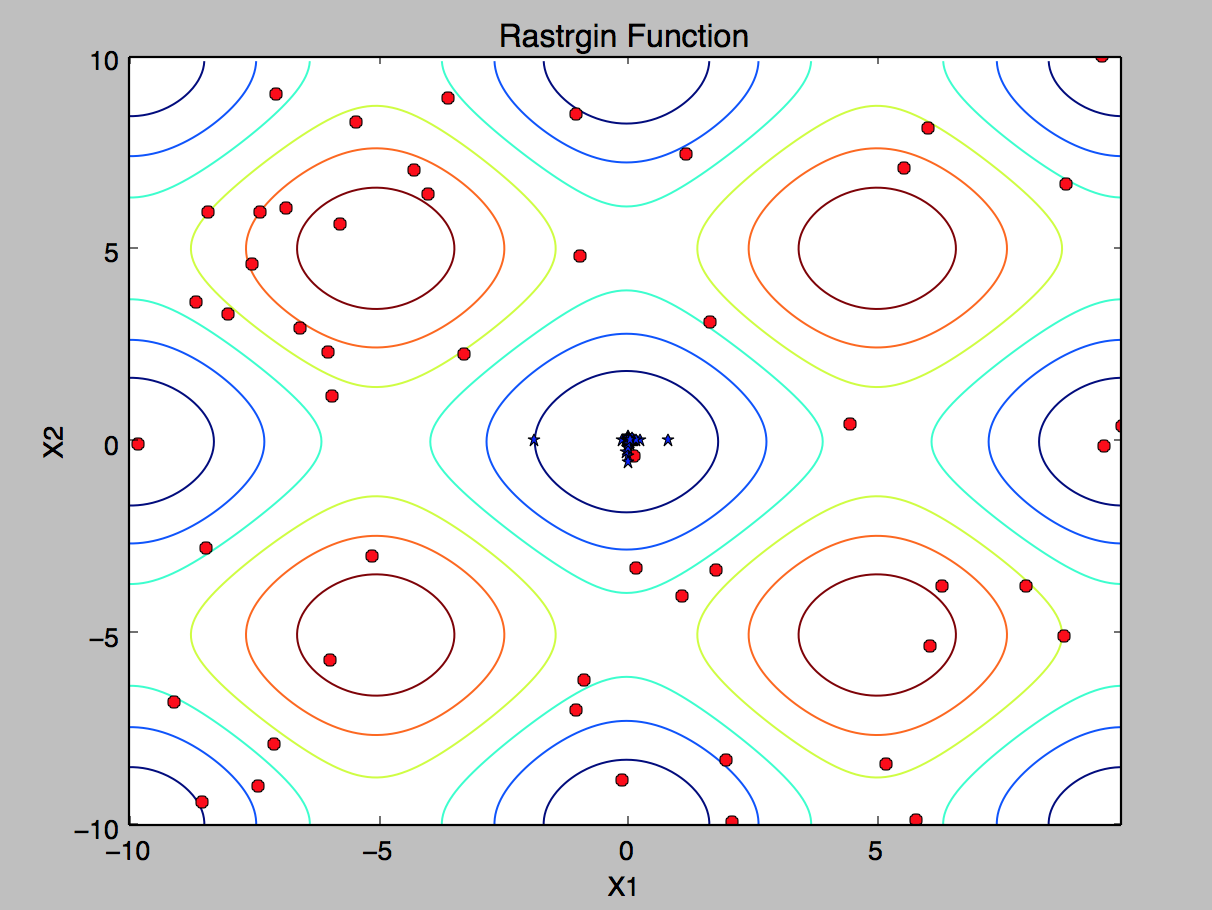
\includegraphics[width=0.7\textwidth]{PSO} 
\centering
\caption{PSO Algorithm (problem 2): circle points are randomly generated 50 initial points. Stars indicate the positions after 50 iterations. }

\end{figure}

\begin{figure}[h]
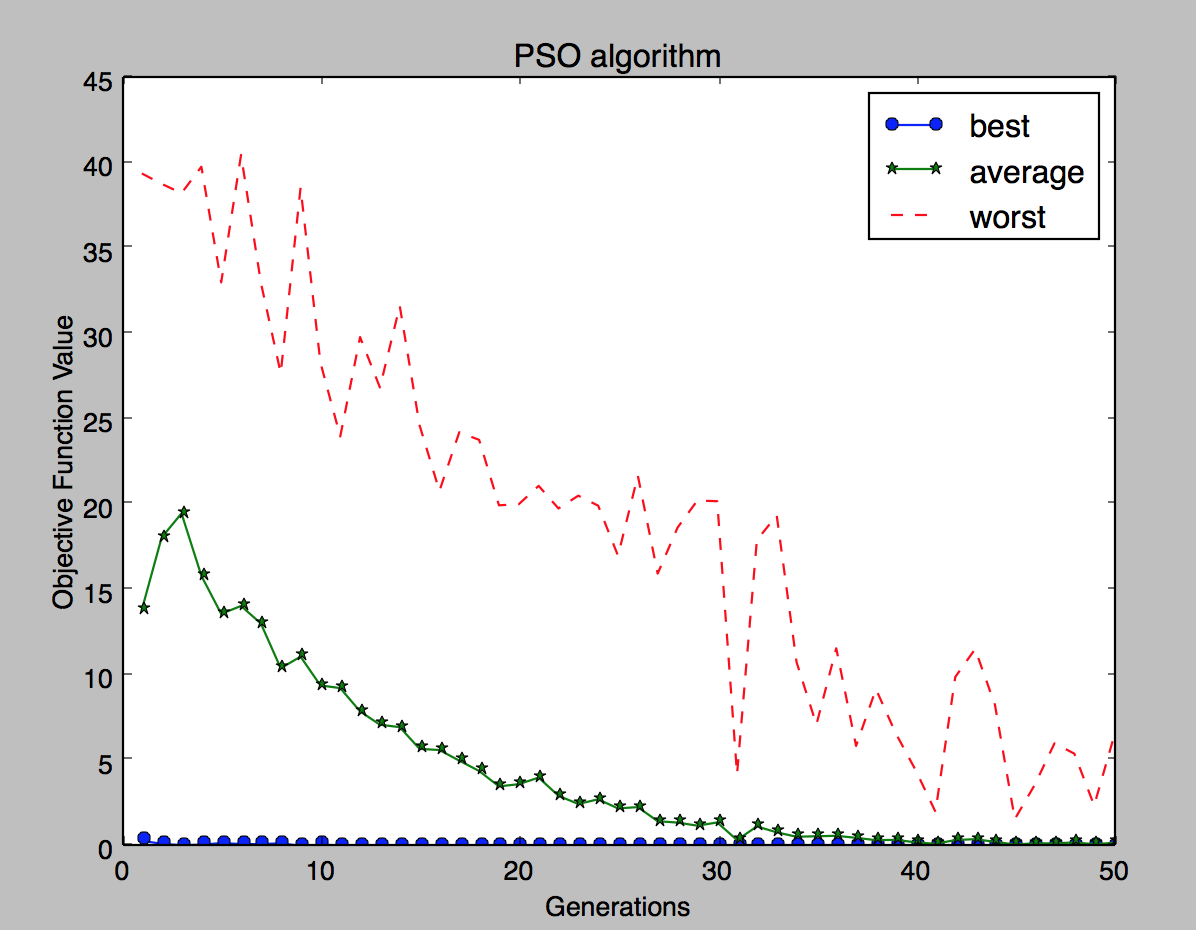
\includegraphics[width=0.7\textwidth]{PSO_min_best} 
\centering
\caption{PSO Algorithm (problem 2): plots of the best, average, and the worst objective function values in the population for 50 generations }

\end{figure}


\subsection*{{Problem 3: }}

Using PSO algorithm, we can find the maximizer: \\
\begin{align*}
x_0 & =  -5.02482780601\\
x_1 & =  5.02524813509\\
f(x_0,x_1) & = -40.5025451078 
\end{align*}
In fact, there are several other global maximizers. PSO method will converge to different global maximizer depending on the initial points which are randomly chosen.   
\begin{figure}[h]
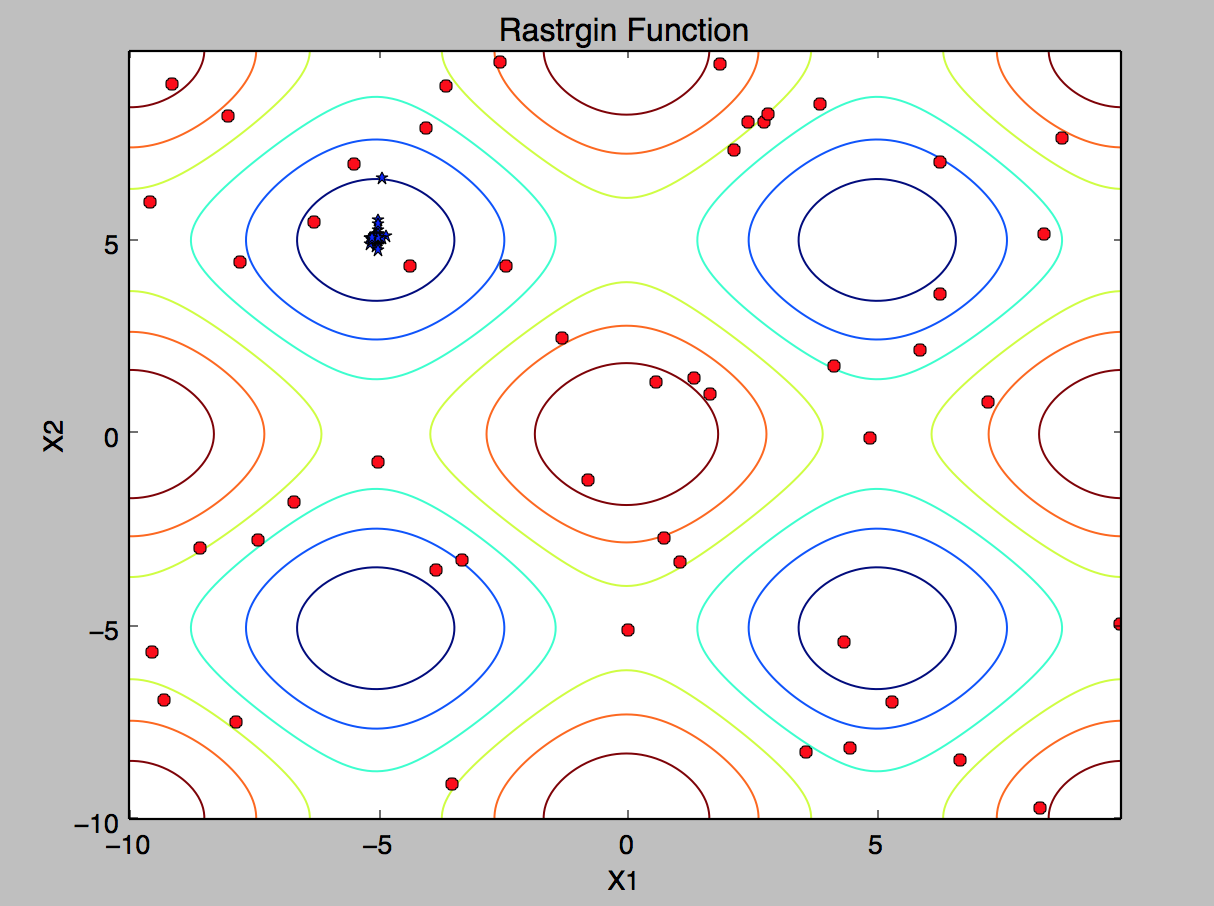
\includegraphics[width=0.7\textwidth]{PSO_max} 
\centering
\caption{PSO Algorithm (problem 3): circle points are randomly generated 50 initial points. Stars indicate the positions after 50 iterations. }

\end{figure}

\begin{figure}[h]
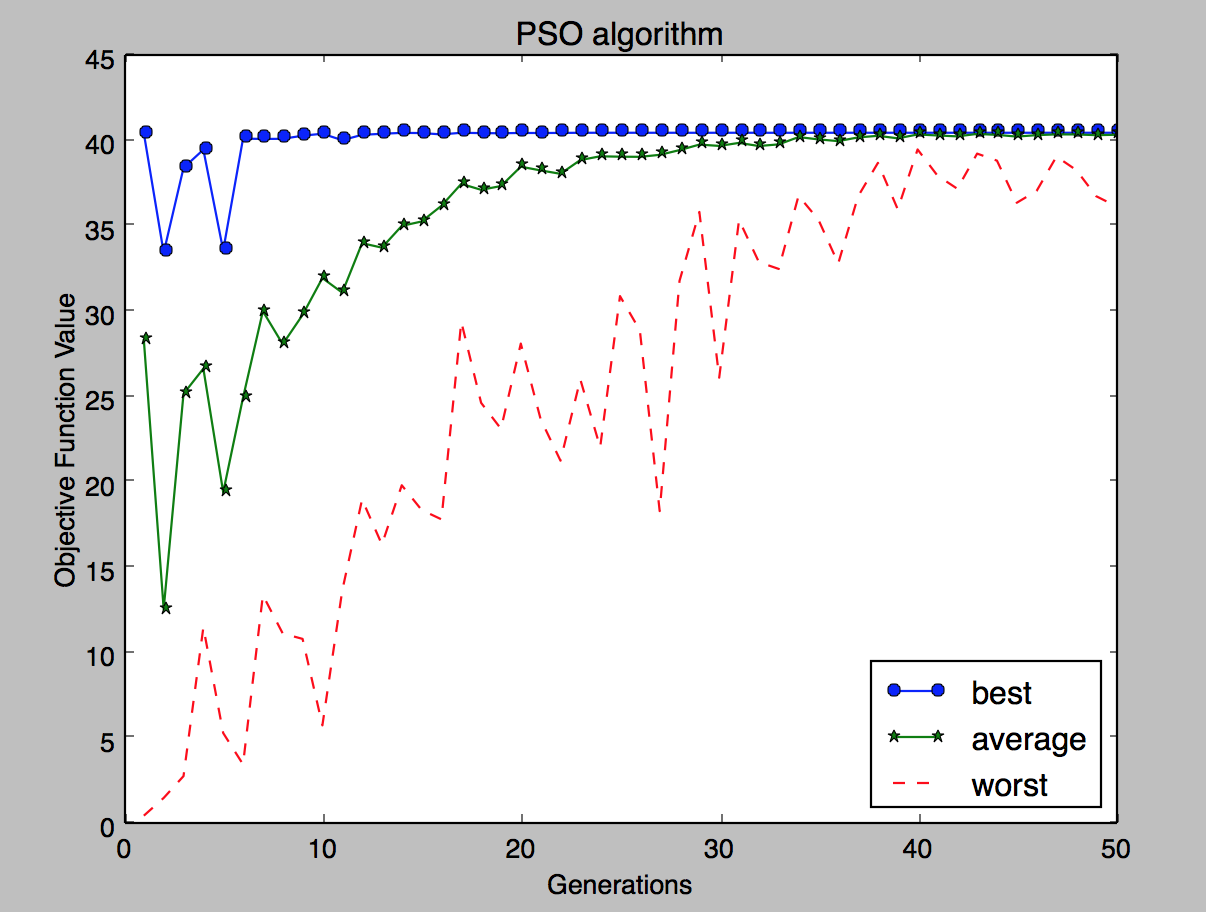
\includegraphics[width=0.7\textwidth]{PSO_max_best} 
\centering
\caption{PSO Algorithm (problem 3): plots of the best, average, and the worst objective function values in the population for 50 generations }

\end{figure}





\subsection*{{Problem 4: }}

Population size:  50  \\
Number of iterations:  50 \\ 
For canonical number genetic algorithm, the minimizer is: \\
\begin{align*}
x_1 & = 0.0408935546875 \\
x_2 & = 0.0390625  \\
f(x_1,x_2)  & = 0.00634456702034
\end{align*}

For real number genetic algorithm, the minimizer is : \\
\begin{align*} 
x_1 & = 0.018313265874 \\
x_2 & = 0.0286761643909 \\
f(x_1, x_2) & = 0.00229673023909
\end{align*} 

\begin{figure} [h]
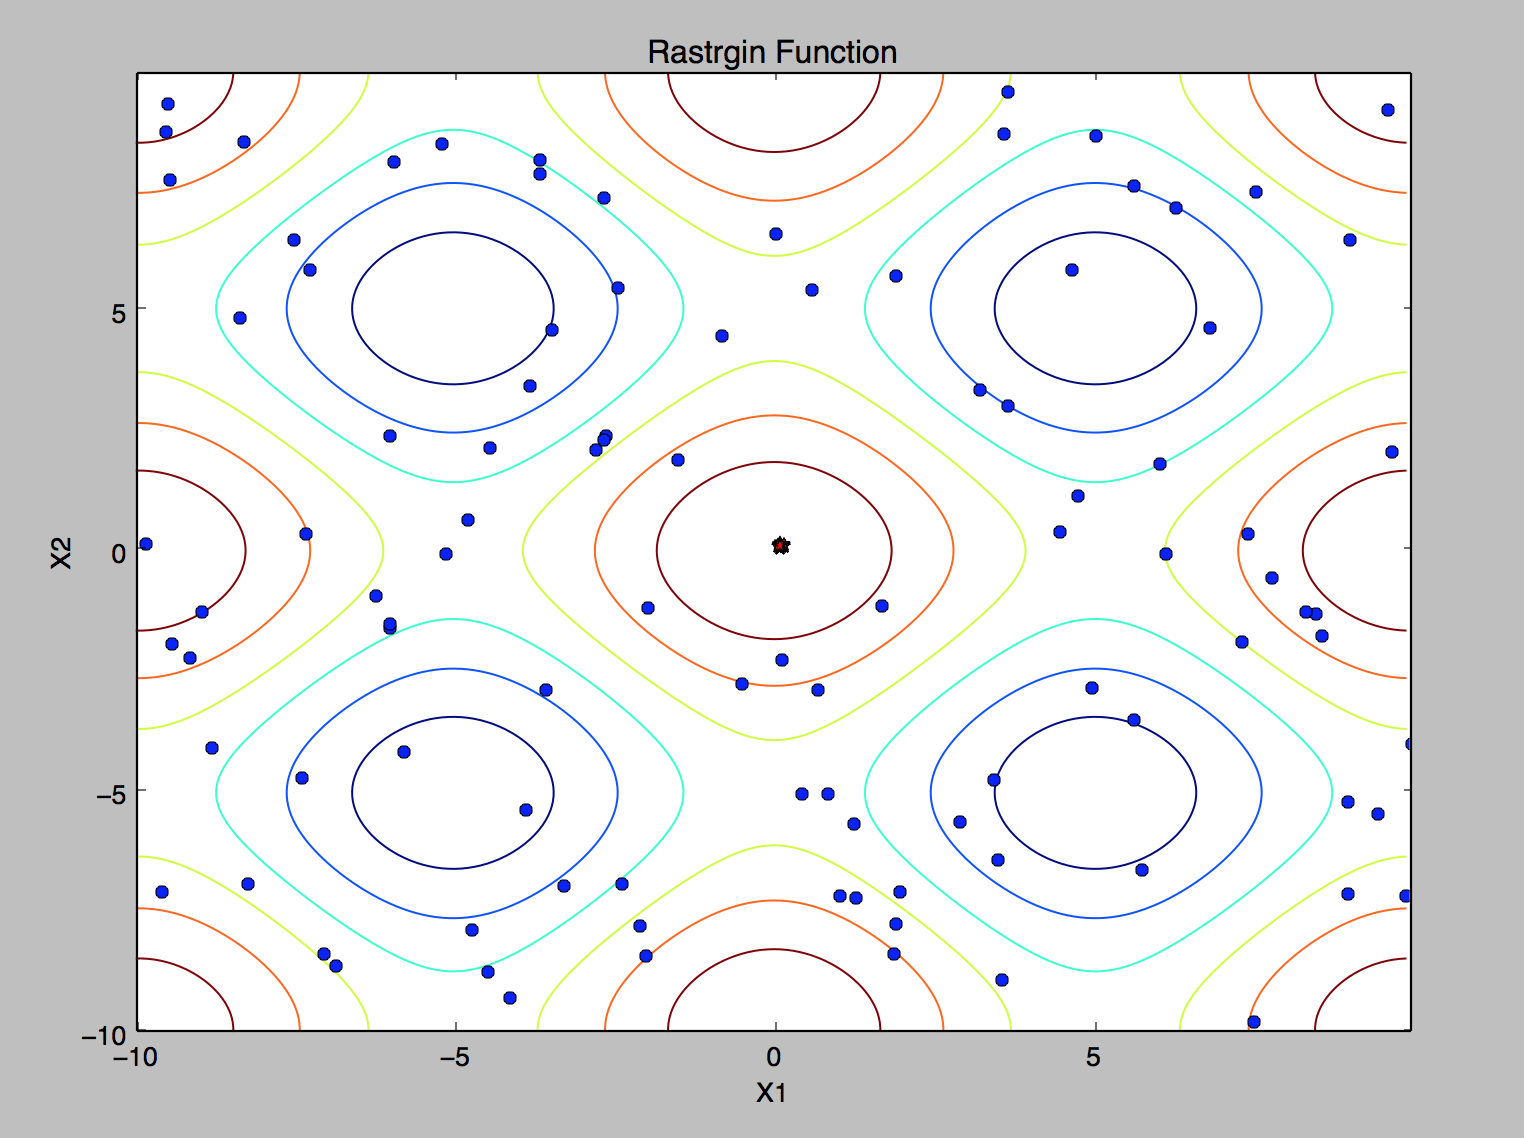
\includegraphics[width=0.7\textwidth]{GA_canonical}
\centering
\caption{Canonical Genetic Algorithm (problem 4): circle points are randomly generated 50 initial points. Stars indicate the positions after 50 iterations. }

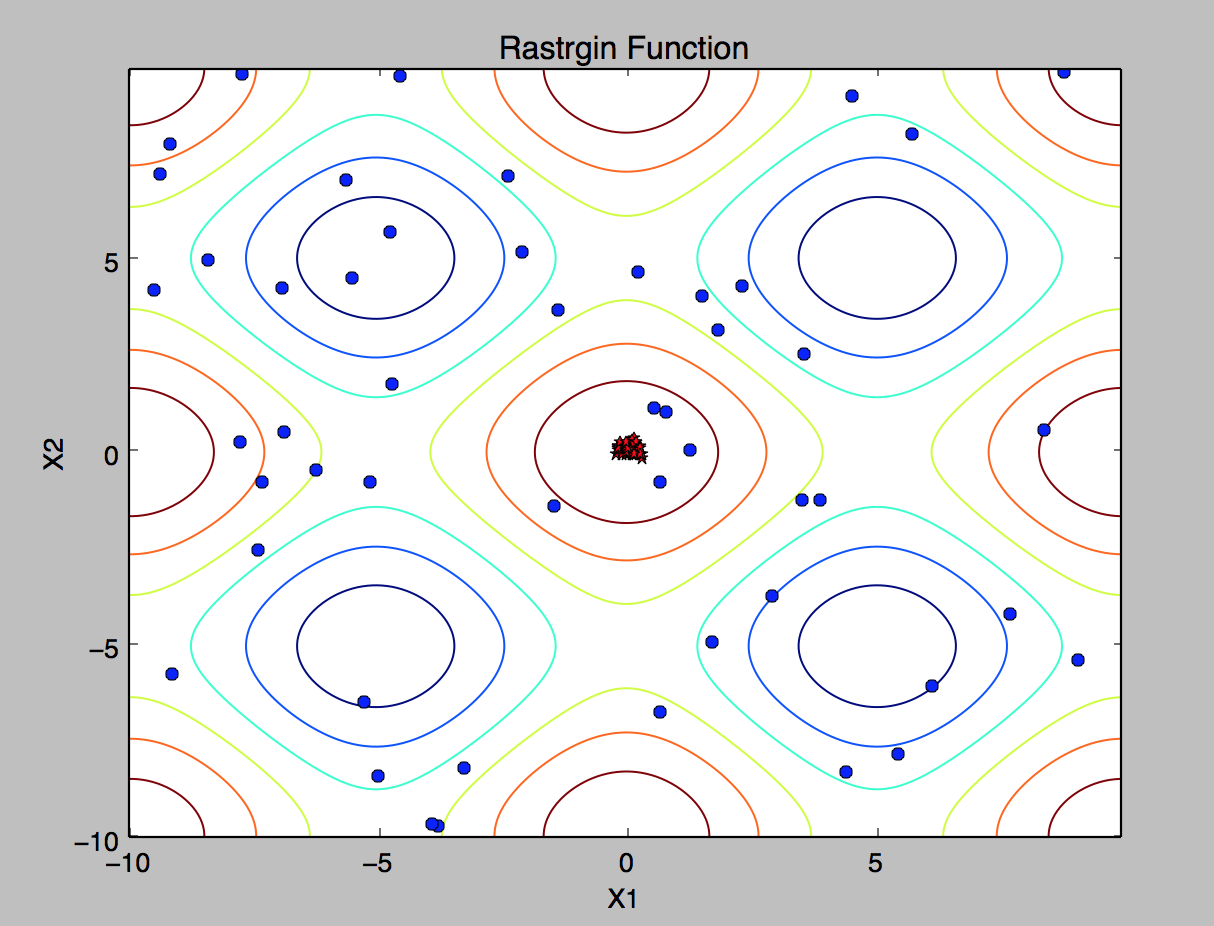
\includegraphics[width=0.7\textwidth]{GA_real_number}
\centering
\caption{Real Number Genetic Algorithm (problem 4): circle points are randomly generated 50 initial points. Stars indicate the positions after 50 iterations. }

\end{figure}

\begin{figure}[h]
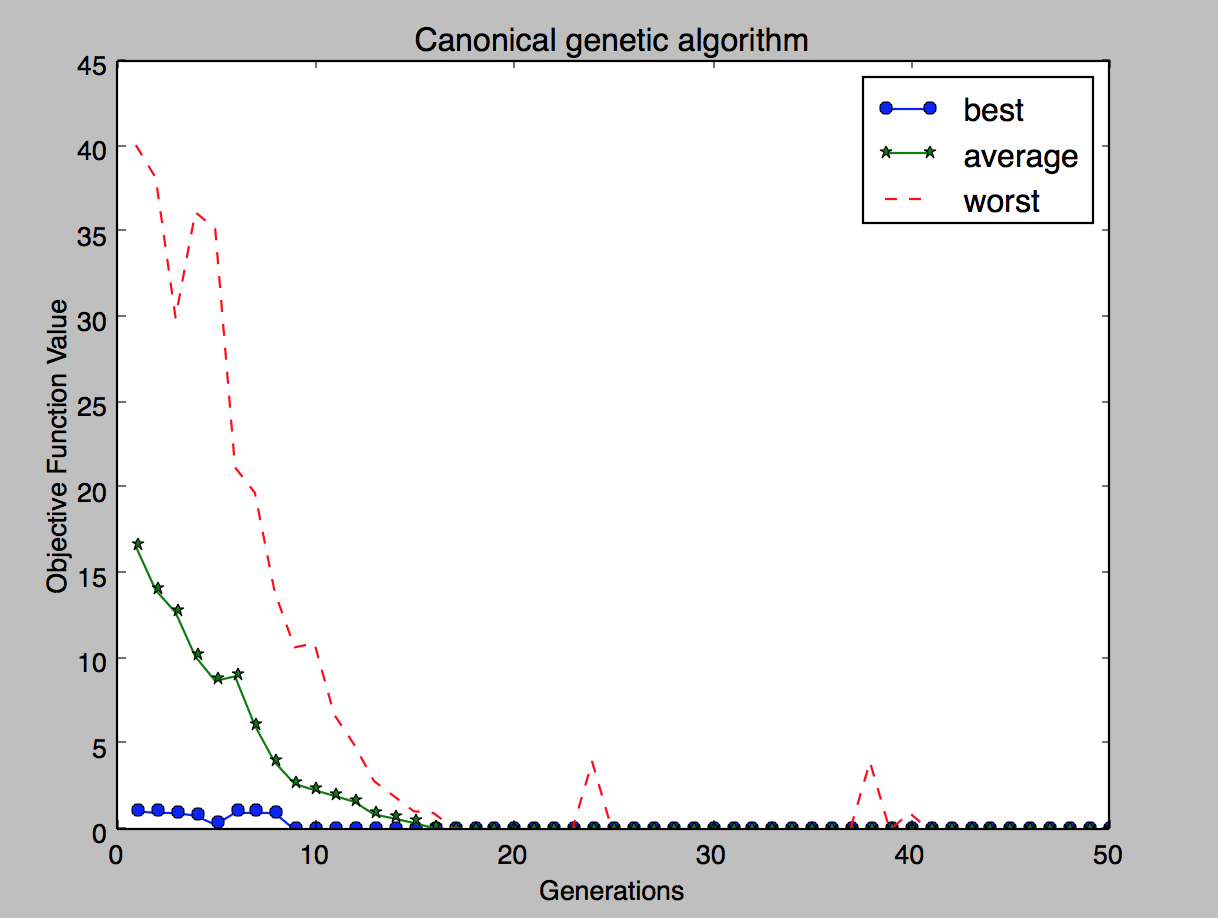
\includegraphics[width=0.7\textwidth]{Canonical_GA_best_plot}
\centering
\caption{Canonical Genetic Algorithm (problem 4): plots of the best, average, and the worst objective function values in the population for 50 generations}


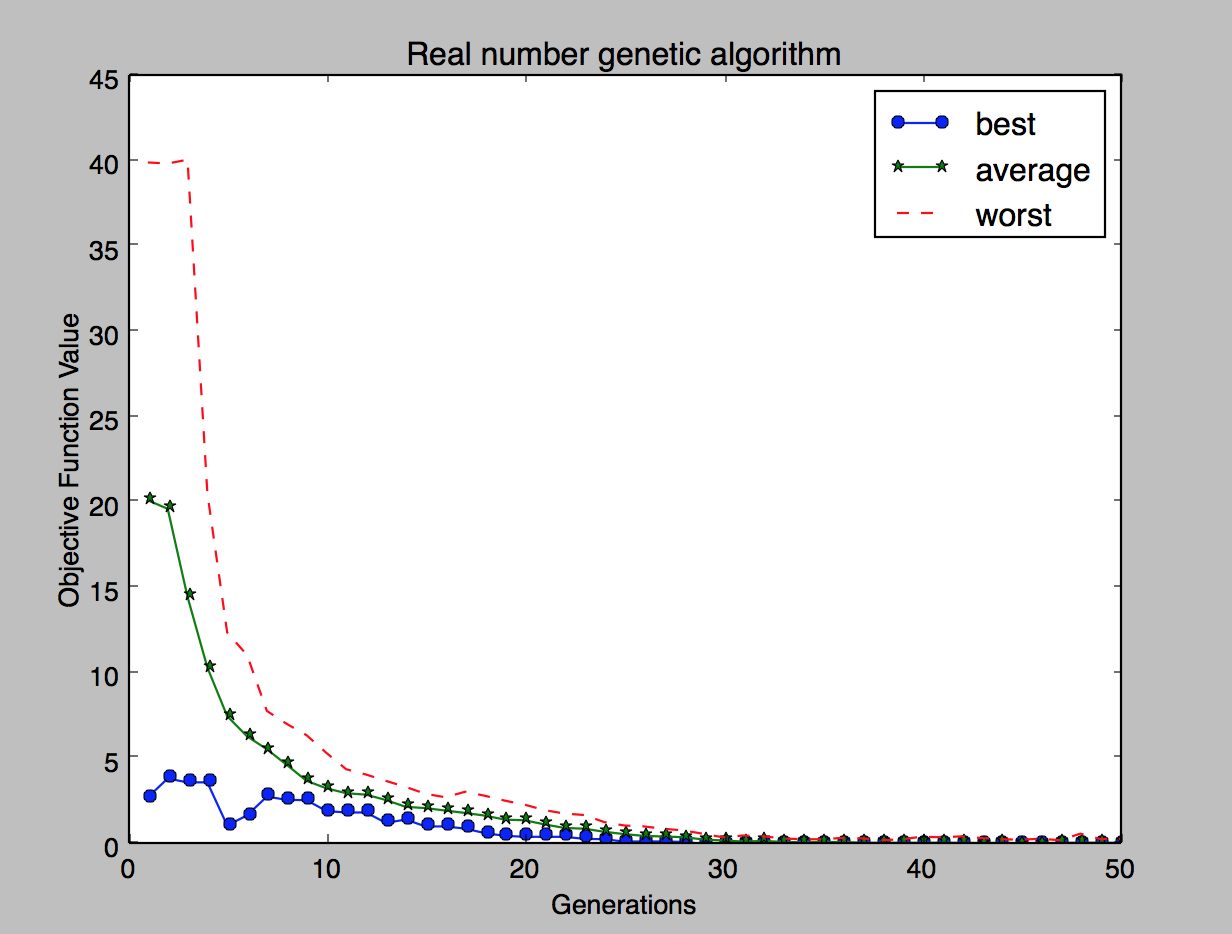
\includegraphics[width=0.7\textwidth]{Real_number_GA}
\centering
\caption{Real Number Genetic Algorithm (problem 4): plots of the best, average, and the worst objective function values in the population for 50 generations}
\end{figure}


\subsection*{{Problem 5: }}

The shortest path is shown in Figure \ref{fig:tsp1}, and the shortest distance is : $37.7222579198$

\begin{figure}[h]
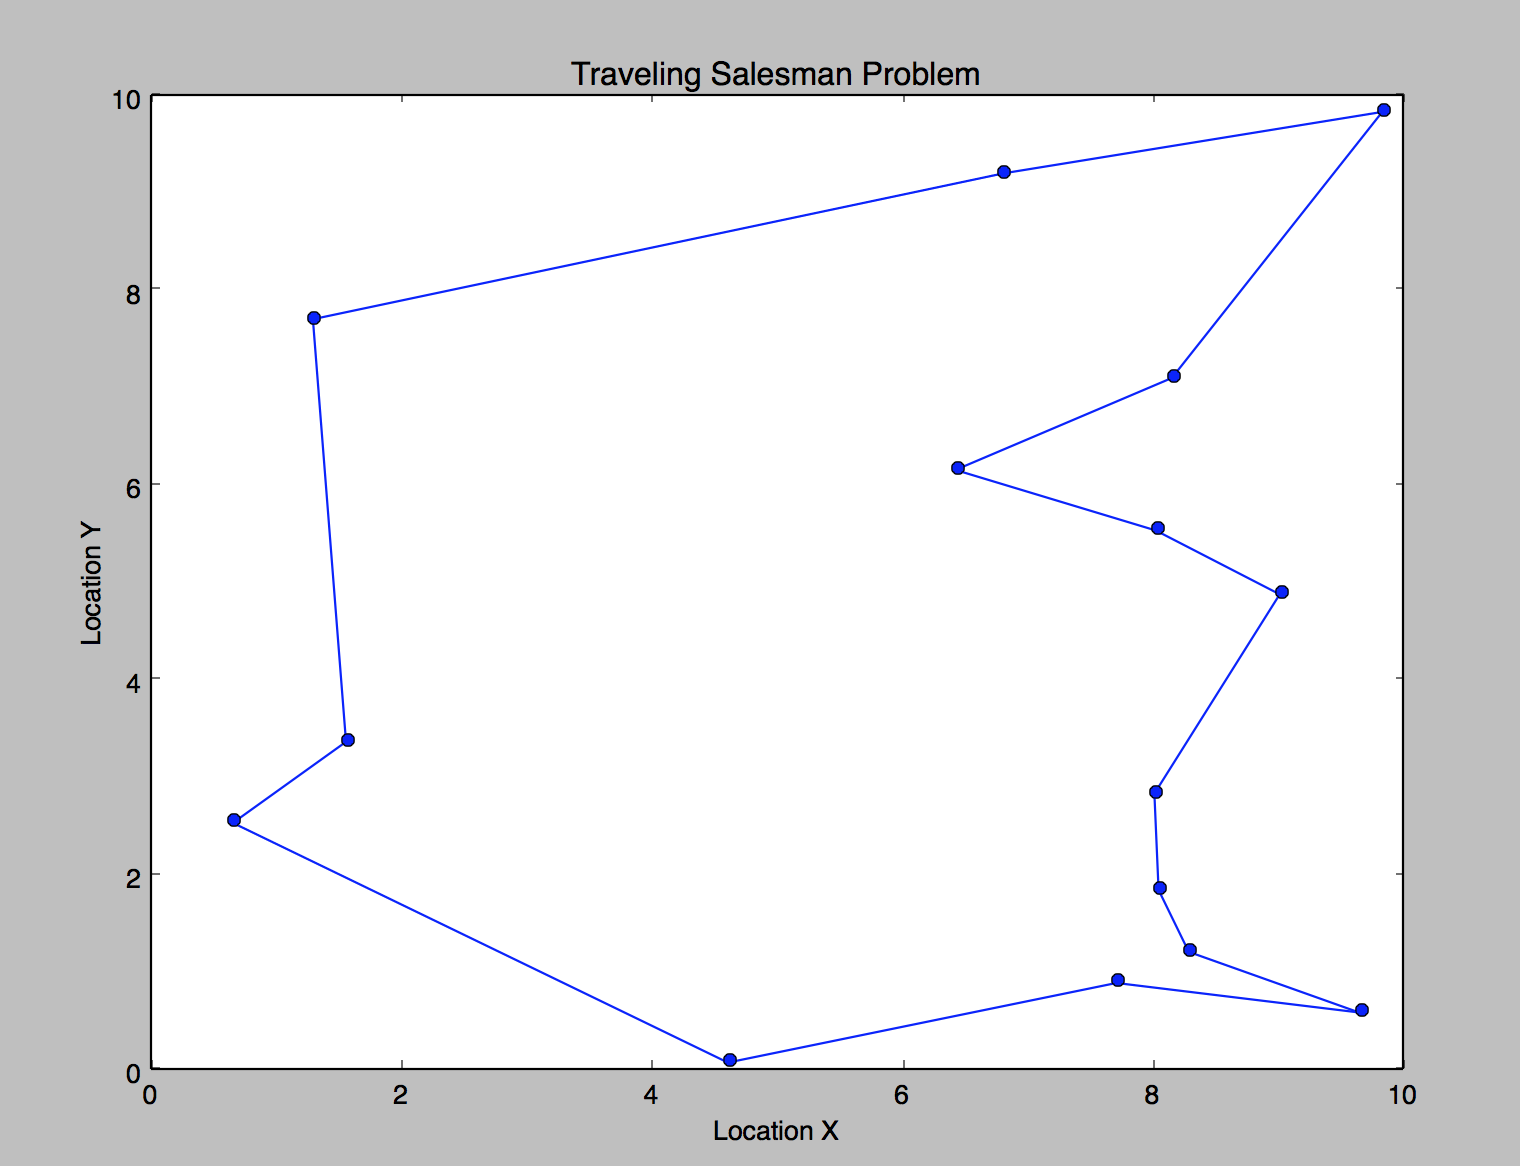
\includegraphics[width=0.7\textwidth]{Traveling_salesman_path}
\centering
\caption{Traveling salesman problem (problem 5): plots of the shortest distance path}
\label{fig:tsp1}

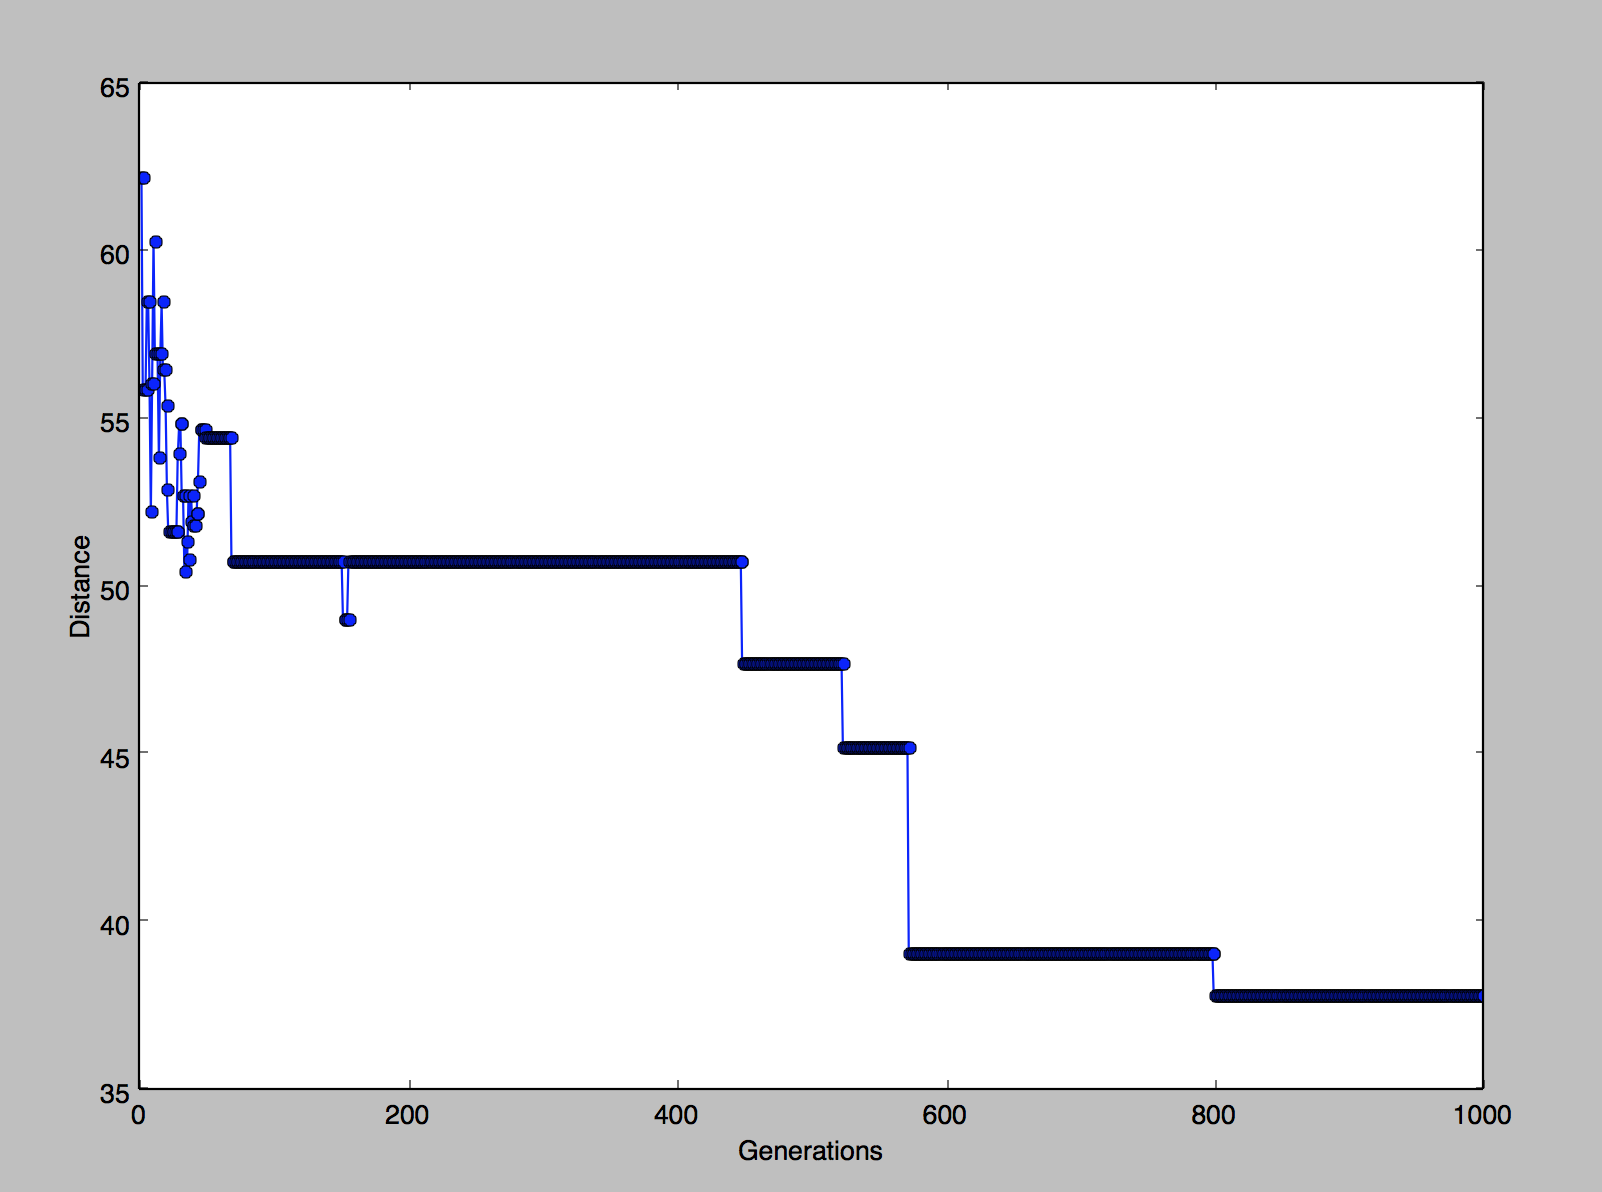
\includegraphics[width=0.7\textwidth]{Distance_vs_generation}
\label{fig:tsp2}
\centering
\caption{Traveling salesman problem (problem 5): plots of the shortest distance for different combinations of the population for 1000 generations}

\end{figure}

\subsection*{{Problem 6: }}


Matlab code for Problem 6: \\
\begin{lstlisting} 
f = [7  10  14  8   7   11  12  6   5   8   15  9   ]; 
A = [];
b = [];
Aeq = [1    1   1   1	0   0   0   0   0   0   0   0; 
       0    0   0   0    1    1   1   1    0   0   0   0 ; 
       0    0   0   0    0    0   0   0    1    1   1   1; 
       1    0   0   0    1    0   0   0    1    0   0   0; 
       0    1   0   0    0    1   0   0    0    1   0   0 ; 
       0    0   1   0    0    0   1   0    0    0   1   0 ;   
       0    0   0   1    0    0   0   1    0    0   0   1  ]; 
beq = [30   40  30  20  20  25  35];
lb = [0, 0, 0, 0, 0, 0, 0, 0, 0, 0, 0, 0]; 
ub = [] ; 
x = linprog(f, A, b, Aeq, beq, lb, ub) 
\end{lstlisting}
The output: 
\begin{lstlisting}
x =

    4.8834
    5.1166
    8.7304
   11.2696
    0.0000
    0.0000
   16.2696
   23.7304
   15.1166
   14.8834
    0.0000
    0.0000
\end{lstlisting}

Code problem2: 
\begin{lstlisting} 
import matplotlib.pyplot as plt
import numpy as np
import sys

import numpy as np
def func(x1, x2):
    return -20 - 0.01*x1**2 - 0.01*x2**2 \
           + 10*(np.cos(0.2*np.pi*x1)+np.cos(0.2*np.pi*x2))


def plotContour(ax, xlim, ylim):
    delta = 0.1
    x = np.arange(xlim[0], xlim[1], delta)
    y = np.arange(ylim[0], ylim[1], delta)
    X1, X2 = np.meshgrid(x, y)
    Z = func(X1,X2)
    ax.set_title("Rastrgin Function")
    ax.set_xlabel("X1")
    ax.set_ylabel("X2")
    cs = ax.contour(X1, X2, Z)
    return cs

def getGbest(p0, p1):
    # find the global best from the personal best.
    f = []
    for i in range(len(p0)):
        f.append(func(p0[i], p1[i]))
    gBest = min(f)
    ind = np.argmin(f)
    g0 = p0[ind]
    g1 = p1[ind]

    return gBest, g0, g1

def init(ax, n):
    #n = 100
    x0 = 20* (np.random.rand(n)-0.5)
    x1 = 20* (np.random.rand(n)-0.5)
    # personal best
    p0 = x0
    p1 = x1

    v0 = 0.1*np.random.rand(n)
    v1 = 0.1*np.random.rand(n)
    gBest, g0, g1 = getGbest(p0, p1)
    ax.plot(x0, x1, 'or')
    pBest = []
    for i in range(n):
        pBest.append(func(x0[i], x1[i]))
    return x0, x1, v0, v1, p0,p1,pBest, g0, g1, gBest

def getBestPlot(x0_dec, x1_dec):

    f = []
    for i in range(len(x0_dec)):
        f.append(func(x0_dec[i], x1_dec[i]))
    best = min(f)
    worst = max(f)
    ave = np.mean(f)
    ind = np.argmin(f)
    return ind, best, worst, ave

def clampVelocity(vCurr, vmax):
    return  min(vmax, max(-vmax, vCurr))

def pmo(ax):
    n =50
    c1 = 2.01
    c2 = 2.09
    bestList = []
    worstList = []
    aveList = []
    counter = []
    x0, x1, v0, v1, p0,p1,pBest,  g0, g1, gBest  = init(ax, n )

    k = 0.729

    vmax = 4.0
    for i in range(50):

        r0 = np.random.rand(n)
        r1 = np.random.rand(n)
        s0 = np.random.rand(n)
        s1 = np.random.rand(n)
        for j in range(n):
            v0[j] = k*(v0[j] + c1*r0[j]*(p0[j]-x0[j])+ c2*s0[j]*(g0-x0[j]))
            v1[j] = k*(v1[j] + c1*r1[j]*(p1[j]-x1[j])+ c2*s1[j]*(g1-x1[j]))
            # clamping velocity
            v0[j] = min(vmax, max(-vmax, v0[j]))
            v1[j] = min(vmax, max(-vmax, v1[j]))

            x0[j] = x0[j] + v0[j]
            x1[j] = x1[j] + v1[j]
            val = func(x0[j], x1[j])
            if val<= pBest[j]:
                pBest[j] = val
                p0[j] = x0[j]
                p1[j] = x1[j]


        gCurrBest, g0Curr, g1Curr = getGbest(p0, p1)
        #print g0Curr, g1Curr,gCurrBest, func(g0Curr, g1Curr)
        if gCurrBest < gBest:
            gBest = gCurrBest
            g0 = g0Curr
            g1 = g1Curr
            print "gBest", g0, g1, gBest, func(g0, g1)

        ind, best, worst, ave  = getBestPlot(x0, x1)
        counter.append(i+1)
        bestList.append(-best)
        worstList.append(-worst)
        aveList.append(-ave)
    ax.plot(x0, x1, "*b")
    fig2 = plt.figure()
    ax1 = fig2.add_subplot(111)
    ax1.plot(counter, bestList, '-o',label='best')
    ax1.plot(counter, aveList, '-*', label = 'average')
    ax1.plot(counter, worstList, '--', label='worst')
    ax1.set_xlabel("Generations")
    ax1.set_ylabel("Objective Function Value")
    ax1.set_title("PSO algorithm")
    ax1.legend(loc=4)
    plt.show()

def main():
    f, (ax) = plt.subplots(1,1, sharex=False)
    plotContour(ax, [-10,10] , [-10,10])
    pmo(ax)
    plt.show()
\end{lstlisting} 

Canonical GA algorithm (problem 4) code : \\
\begin{lstlisting} 
import matplotlib.pyplot as plt
import numpy as np
from random import sample
def func(x1, x2):
    return -20 - 0.01*x1**2 - 0.01*x2**2 \
           + 10*(np.cos(0.2*np.pi*x1)+np.cos(0.2*np.pi*x2))

def plotContour(ax, xlim, ylim):
    delta = 0.1
    x = np.arange(xlim[0], xlim[1], delta)
    y = np.arange(ylim[0], ylim[1], delta)
    X1, X2 = np.meshgrid(x, y)
    Z = func(X1,X2)
    ax.set_title("Rastrgin Function")
    ax.set_xlabel("X1")
    ax.set_ylabel("X2")
    cs = ax.contour(X1, X2, Z)
    return cs


def mapping(binNum, n):
    decVal = 20.0 * binNum/(np.power(2, n-1)) -10
    return decVal

def init(ax, n):
    x0_dec = []
    x1_dec = []
    L = 32
    max = np.power(2, L/2-1)
    x0_bin = np.random.randint(0, max, size=n)
    x1_bin = np.random.randint(0, max, size=n)
    for i in range(n):
        x0_dec.append(mapping(x0_bin[i], L/2))
        x1_dec.append(mapping(x1_bin[i], L/2))

    ax.plot(x0_dec, x1_dec, 'ob')
    return x0_bin, x1_bin, x0_dec, x1_dec

def selection(x0_bin, x1_bin, x0_dec, x1_dec, k):
    f = []
    for i in range(len(x0_dec)):
        f.append(func(x0_dec[i], x1_dec[i]))
    base = min(f)
    f = [x-base for x in f]
    cumSum = np.cumsum(f)
    new_x0_dec = []
    new_x1_dec = []
    new_x0_bin = []
    new_x1_bin = []
    f_index = [0] * k

    alpha = np.random.rand(k)*sum(f)
    for i in range(k):
        for j in range(len(x0_dec)):
            if alpha[i]> cumSum[j]:
                f_index[i] += 1
            else:
                break

    for index in f_index:
        new_x0_dec.append(x0_dec[f_index[index]])
        new_x1_dec.append(x1_dec[f_index[index]])
        new_x0_bin.append(x0_bin[f_index[index]])
        new_x1_bin.append(x1_bin[f_index[index]])
    return new_x0_bin, new_x1_bin, new_x0_dec, new_x1_dec


def crossover(x0_bin, x1_bin, x0_dec, x1_dec, n):

    pc = 0.65
    pm = 0.0075

    # choosing crossing site;
    N = 2* int(pc *  n/2)   #  number of parents who are ready to do crossover.
    L = 32
    parent_index =  sample(xrange(len(x0_dec)), N)
    i=0
    while i<len(parent_index):
        parent1 = "{0:b}".format( x0_bin[parent_index[i]]*np.power(2, L/2) + x1_bin[parent_index[i]]).zfill(L)
        parent2 = "{0:b}".format( x0_bin[parent_index[i+1]]*np.power(2, L/2)+ x1_bin[parent_index[i+1]]).zfill(L)
        site = np.random.randint(0,L-1)
        child1 = parent1[0:site] + parent2[site:L]
        child2 = parent2[0:site] + parent1[site:L]


        x0_bin[parent_index[i]]  =  int(child1[0:L/2], 2)
        x0_bin[parent_index[i+1]]=  int(child2[L/2:L], 2)
        x1_bin[parent_index[i]]  =  int(child1[L/2:L], 2)
        x1_bin[parent_index[i+1]]=  int(child2[0:L/2], 2)
        i+=2

    ## Mutation
    for i in range(len(x0_bin)):
        s = "{0:b}".format(x0_bin[i]).zfill(L/2)
        new_s = ""
        for j in range(len(s)):
            val = np.random.rand()
            if val < pm:
                new_s += str(1- int(s[j]))
            else:
                new_s += s[j]
        x0_bin[i] = int(new_s, 2)

        s1 = "{0:b}".format(x1_bin[i]).zfill(L/2)
        new_s1 = ""
        for j in range(len(s1)):
            val = np.random.rand()
            if val < pm:
                new_s1 += str(1- int(s1[j]))
            else:
                new_s1 += s1[j]

        x1_bin[i] = int(new_s1, 2)

    #update x0_dec and x1_dec:
    for i in range(len(x0_bin)):
        x0_dec[i]  = mapping(x0_bin[i], L/2)
        x1_dec[i]  = mapping(x1_bin[i], L/2)


    return x0_bin, x1_bin, x0_dec, x1_dec

def getBestPlot(x0_dec, x1_dec):

    f = []
    for i in range(len(x0_dec)):
        f.append(-func(x0_dec[i], x1_dec[i]))
    best = min(f)
    worst = max(f)
    ave = np.mean(f)
    ind = np.argmin(f)
    return ind, best, worst, ave

def ga(ax):
    n = 50   #  number of initial points.
    bestList = []
    worstList = []
    aveList = []
    counter = []

    x0_bin, x1_bin, x0_dec, x1_dec = init(ax, n)

    for i in range(50):
        x0_bin, x1_bin, x0_dec, x1_dec = selection(x0_bin, x1_bin, x0_dec, x1_dec, k=len(x0_dec))
        x0_bin, x1_bin, x0_dec, x1_dec = crossover(x0_bin, x1_bin, x0_dec, x1_dec, n)  # crossover and mutation

        ind, best, worst, ave  = getBestPlot(x0_dec, x1_dec)

        counter.append(i+1)
        bestList.append(best)
        worstList.append(worst)
        aveList.append(ave)

    print x0_dec[ind], x1_dec[ind], -func(x0_dec[ind], x1_dec[ind])
    plt.plot(x0_dec, x1_dec, '*r')

    fig2 = plt.figure()
    ax1 = fig2.add_subplot(111)
    ax1.plot(counter, bestList, '-o',label='best')
    ax1.plot(counter, aveList, '-*', label = 'average')
    ax1.plot(counter, worstList, '--', label='worst')
    ax1.set_xlabel("Generations")
    ax1.set_ylabel("Objective Function Value")
    ax1.set_title("Canonical genetic algorithm")
    ax1.legend()
    plt.show()

def main():
    f, (ax) = plt.subplots(1,1, sharex=False)
    plotContour(ax, [-10,10] , [-10,10])
    ga(ax)
    plt.show()

if  __name__ == "__main__":
    main()
\end{lstlisting}

Real number GA algorithm: \\
\begin{lstlisting} 
import matplotlib.pyplot as plt
import numpy as np
from random import sample
def func(x1, x2):
    return -20 - 0.01*x1**2 - 0.01*x2**2 \
           + 10*(np.cos(0.2*np.pi*x1)+np.cos(0.2*np.pi*x2))


def plotContour(ax, xlim, ylim):
    delta = 0.1
    x = np.arange(xlim[0], xlim[1], delta)
    y = np.arange(ylim[0], ylim[1], delta)
    X1, X2 = np.meshgrid(x, y)
    Z = func(X1,X2)
    ax.set_title("Rastrgin Function")
    ax.set_xlabel("X1")
    ax.set_ylabel("X2")
    cs = ax.contour(X1, X2, Z)
    return cs

def mapping(binNum, n):
    decVal = 20.0 * binNum/(np.power(2, n-1)) -10
    return decVal


def init(ax, n):
    x0_dec = []
    x1_dec = []
    L = 32
    max = np.power(2, L/2-1)
    x0_bin = np.random.randint(0, max, size=n)
    x1_bin = np.random.randint(0, max, size=n)
    for i in range(n):
        x0_dec.append(mapping(x0_bin[i], L/2))
        x1_dec.append(mapping(x1_bin[i], L/2))

    ax.plot(x0_dec, x1_dec, 'ob')
    return x0_bin, x1_bin, x0_dec, x1_dec

def selection(x0_dec, x1_dec, k):
    f = []
    for i in range(len(x0_dec)):
        f.append(func(x0_dec[i], x1_dec[i]))
    base = min(f)
    f = [x-base for x in f]
    cumSum = np.cumsum(f)
    new_x0_dec = []
    new_x1_dec = []
    #new_x0_bin = []
    #new_x1_bin = []
    f_index = [0] * k


    alpha = np.random.rand(k)*sum(f)
    for i in range(k):
        for j in range(len(x0_dec)):
            if alpha[i]> cumSum[j]:
                f_index[i] += 1
            else:

                break

    for index in f_index:
        new_x0_dec.append(x0_dec[f_index[index]])
        new_x1_dec.append(x1_dec[f_index[index]])
        #new_x0_bin.append(x0_bin[f_index[index]])
        #new_x1_bin.append(x1_bin[f_index[index]])
    return  new_x0_dec, new_x1_dec


def crossover(x0_dec, x1_dec, n):

    pc = 0.65
    pm = 0.075

    # choosing crossing site;
    N = 2* int(pc *  n/2)   #  number of parents who are ready to do crossover.
    L = 32
    parent_index =  sample(xrange(len(x0_dec)), N)
    i=0
    while i<len(parent_index):
        parent1_x0 = x0_dec[parent_index[i]]
        parent1_x1 = x1_dec[parent_index[i]]
        parent2_x0 = x0_dec[parent_index[i+1]]
        parent2_x1 = x1_dec[parent_index[i+1]]

        w = np.random.normal(0, 0.1, 4)
        child1_x0  = (parent1_x0+parent2_x0)/2 + w[0]
        child1_x1  = (parent1_x1+parent2_x1)/2 + w[1]
        child2_x0  = (parent1_x0+parent2_x0)/2 + w[2]
        child2_x1  = (parent1_x1+parent2_x1)/2 + w[3]

        x0_dec[parent_index[i]] = child1_x0
        x1_dec[parent_index[i]] = child1_x1
        x0_dec[parent_index[i+1]] = child2_x0
        x1_dec[parent_index[i+1]] = child2_x1
        i+=2
    ## Mutation
    for i in range(len(x0_dec)):
        val = np.random.rand()

        if val < pm :
            w = np.random.normal(0, 0.1, 2)
            x0_dec[i] += w[0]
            x1_dec[i] += w[1]
    return  x0_dec, x1_dec

def getBestPlot(x0_dec, x1_dec):

    f = []
    for i in range(len(x0_dec)):
        f.append(-func(x0_dec[i], x1_dec[i]))
    best = min(f)
    worst = max(f)
    ave = np.mean(f)
    ind = np.argmin(f)
    return ind, best, worst, ave

def ga(ax):
    n = 50   #  number of initial points.

    bestList = []
    worstList = []
    aveList = []
    counter = []

    x0_bin, x1_bin, x0_dec, x1_dec = init(ax, n)

    for i in range(50):
        x0_dec, x1_dec = selection(x0_dec, x1_dec, k=len(x0_dec))
        x0_dec, x1_dec = crossover(x0_dec, x1_dec, n)  # crossover and mutation
        ind, best, worst, ave  = getBestPlot(x0_dec, x1_dec)

        counter.append(i+1)
        bestList.append(best)
        worstList.append(worst)
        aveList.append(ave)
    print x0_dec[ind], x1_dec[ind], -func(x0_dec[ind], x1_dec[ind])
    plt.plot(x0_dec, x1_dec, '*r')

    fig2 = plt.figure()
    ax1 = fig2.add_subplot(111)
    ax1.plot(counter, bestList, '-o',label='best')
    ax1.plot(counter, aveList, '-*', label = 'average')
    ax1.plot(counter, worstList, '--', label='worst')
    ax1.set_xlabel("Generations")
    ax1.set_ylabel("Objective Function Value")
    ax1.set_title("Real number genetic algorithm")
    ax1.legend()
    plt.show()

def main():
    f, (ax) = plt.subplots(1,1, sharex=False)
    plotContour(ax, [-10,10] , [-10,10])
    ga(ax)
    plt.show()

\end{lstlisting}

Traveling salesman problem (problem 5):
\begin{lstlisting} 

import matplotlib.pyplot as plt
import numpy as np
import random
from random import shuffle
import sys

def getDist(comb):
    locX = zip(*comb)[0]
    locY = zip(*comb)[1]
    dist = 0
    for i in range(len(locX)-1):
        dx = locX[i]-locX[i+1]
        dy = locY[i]-locY[i+1]
        dist += np.sqrt(dx**2+dy**2)
    dist += np.sqrt((locX[-1]-locX[0])**2 + (locY[-1]-locY[0])**2)

    return dist

def plotConnection(comb):
    locX = zip(*comb)[0]
    locY = zip(*comb)[1]
    for i in range(len(locX)-1):
        plt.plot((locX[i], locX[i+1]), (locY[i], locY[i+1]), 'o-b')
    plt.plot((locX[0], locX[-1]), (locY[0], locY[-1]), 'o-b')
    plt.xlabel("Location X")
    plt.ylabel("Location Y")
    plt.title("Traveling Salesman Problem")
    plt.show()


def switchByIndex(ind1, ind2, List):
    temp = List[ind2]
    List[ind2] = List[ind1]
    List[ind1] = temp

    return List

def init(locX, locY, num):
    zList = []
    for i in range(num):
        z = zip(locX, locY)
        shuffle(z)
        zList.append(z)
    return zList

def listInsert(l, l1,  pivot):
    # insert l1 into l starting from pivot points:
    assert (pivot<len(l))
    new_list = []
    for i in range(pivot):
        new_list.append(l[i])

    new_list.extend(l1)
    for i in np.arange(pivot, len(l)):
        new_list.append(l[i])
    return new_list

def selection(zList):
    f = []
    k = len(zList)
    for comb in zList:
        f.append(-getDist(comb))
    base = min(f)
    f = [x-base for x in f]
    cumSum = np.cumsum(f)
    alpha = np.random.rand(k)*sum(f)
    f_index = [0]* k
    for i in range(len(alpha)):
        for j in range(len(cumSum)):
            if alpha[i] > cumSum[j]:
                 f_index[i] += 1
            else:
                break
    new_zList =[]
    for ind in f_index:
        new_zList.append(zList[ind])

    return new_zList

def crossover(zList):
    pc = 0.75
    N = int(pc*len(zList)/2)*2   # number of  parents (even number)
    numSub = int(len(zList[0])/3)

    parent_index =  random.sample(xrange(len(zList)), N)
    i=0
    while i<len(parent_index):
        pivot1 = random.sample(xrange(1,len(zList[0])*2/3-1), 1)[0]
        pivot2 = random.sample(xrange(1,len(zList[0])*2/3-1), 1)[0]
        #print pivot
        parent1 = zList[parent_index[i]]
        parent2 = zList[parent_index[i+1]]

        snap1 = [x for x in parent2 if x not in parent1[pivot1: pivot1+numSub]]
        snap2 = [x for x in parent1 if x not in parent2[pivot2: pivot2+numSub]]

        zList[parent_index[i]] = listInsert(snap1, parent1[pivot1:pivot1+numSub], pivot1)
        zList[parent_index[i+1]] = listInsert(snap2, parent2[pivot2:pivot2+numSub], pivot2)

        #print zList[parent_index[i]]
        #print zList[parent_index[i+1]]


        i+=2
    return zList

def mutation(zList):

    pm = 0.0075

    #N = int(pc*len(zList))   # number of single parents.

    for i in range(len(zList)):
        m = np.random.rand()
        #print m
        if m<pm:
            pivot = random.sample(xrange(1,len(zList[0])), 2)
            zList[i] = switchByIndex(pivot[0], pivot[1], zList[i])

    return zList

def GA_algorithm(locX, locY):
    num = 50   # initiate 50 combinations

    zList = init(locX, locY, num)

    counter = []
    best = []

    for i in range(1000):
        counter.append(i+1)
        zList = selection(zList)
        zList = crossover(zList)
        zList = mutation(zList)
        bestDist = sys.maxint
        for comb in zList:
            d = getDist(comb)
            if d<bestDist:
                bestDist = d
                bestPath = comb
        best.append(bestDist)
    print bestDist
    plt.plot(counter, best, '-')
    plt.xlabel("Generations")
    plt.ylabel("Distance")
    plt.show()

    plotConnection(bestPath)
    return locX, locY

def main():

    locX = [7.7176, 9.8397, 1.3001, 4.6141, 9.0204, 1.5651, 6.4311,
            8.0298, 8.2941, 0.6621, 9.6546, 6.8045, 8.0196, 8.1590, 8.0531]
    locY = [0.8955, 9.8352, 7.7070, 0.0784, 4.8838, 3.3703, 6.1604,
            5.5397, 1.2147, 2.5383, 0.5923, 9.2022, 2.8386, 7.1041, 1.8498]
    GA_algorithm(locX, locY)
\end{lstlisting} 



\end{document}
